\documentclass{article}
\usepackage{polski}
\usepackage[utf8]{inputenc}
\usepackage{amsmath}
\usepackage{amsfonts}
\usepackage{mathtools}
\usepackage{multirow}
\usepackage[table,xcdraw]{xcolor}
\usepackage{graphicx}
\usepackage{float}
\usepackage{placeins}
\usepackage[left=2cm,right=2cm,top=2.5cm,bottom=2.5cm]{geometry}

\makeatletter
\newcommand{\mathleft}{\@fleqntrue\@mathmargin0pt}
\newcommand{\mathcenter}{\@fleqnfalse}
\makeatother


\graphicspath{{Grafiki/}}

\title{Modelowanie i sterowanie robotów\\ PROJEKT}
\author{Arkadiusz Piórkowski}

\begin{document}
%\pagenumbering{gobble}
\maketitle

%%%%%%%%%%%%%%%%%%%%%%%%%%%%%%%%%%%%%%%%%%%%%%%%%%%%%%%%%%%%%%%%%%%%%%%%%%%

\section{Zadanie}

Zadaniem projektu jest rozwiązanie zadania prostego i odwrotnego kinematyki robota przedstawionego na rysunku~\ref{fig::robot}.
\begin{figure}[H]
	\centering
	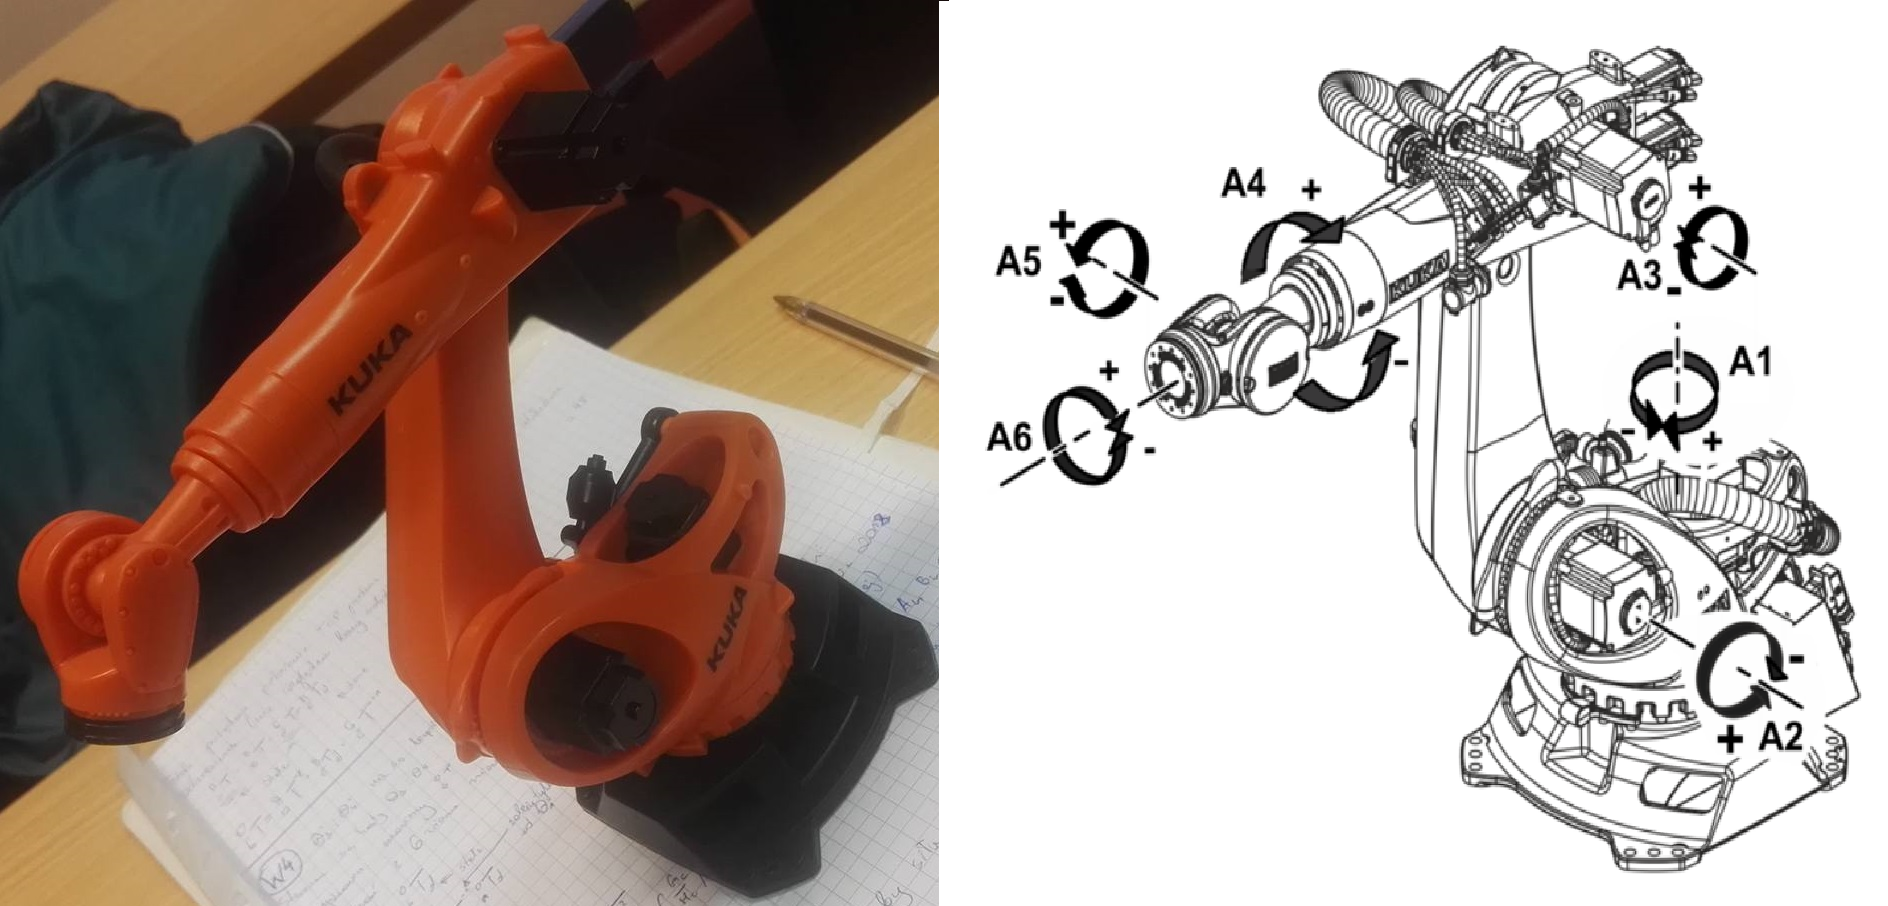
\includegraphics[width=\textwidth]{robot_KUKA_KR_QUANTECpro.png}
	\caption{Robot firmy KUKA serii KR QUANTEC pro}
	\label{fig::robot}
\end{figure}

Proste zadanie kinematyki (PZK) polega na znalezieniu macierzy jednorodnej $ ^0_6 T$ przy znajomo\'sci warto\'sci zmiennych złączowych $\theta_i$.
\newline
Odwrotne zadanie kinematyki (OZK) polega na znalezieniu warto\'sci zmiennych złączowych $\theta_i$ przy znajmo\'sci macierzy jednorodnej  $^0_6 T$.

Przedstawiony manipulator to 6-osiowy robot o strukturze szeregowej. Zatem do rozwiązania wykorzystano algorytm postępowania dla manipulatorów szeregowych przedstawiony podczas wykładu prof. C.Zielińskiego:
\begin{enumerate}
\item Narysować manipulator
\item Wskazać osie obrotu lub translacji (dla złącz obrotowych lub translacyjnych)
\item Przyporządkować osie $_i z$ i-tych układów osiom obrotu/translacji
\item Znaleźć wspólne prostopadłe pomiędzy osiami $_{i-1} z$ i $_i z$ (jeżeli te osie się przecinają, to wspólna prostopadła pokrywa się z $_{i-1} z \times _i z $)
\item Okre\'slić osie $_i x$ - o\'s $_{i-1}x$ pokrywa się ze wspólną prostopadłą do $_{i-1} z$ i $_i z$ (jest skierowana od $_{i-1} z$ do $_i z$)
\item Wyznaczyć osie $_{i}y$ jako $_{i}y = _{i}z \times _{i}x$
\item Układ bazowy 0 powinien być tak ulokowany, aby $\alpha_0, a_0$ i $\theta_1$ lub $d_1$ były równe $0 \Rightarrow _{0}z = _{1}z$ i $_0^0 P = _1^0 P$ 
\item Wyznaczyć parametry złącz i członów 
\begin{itemize}
\item $a_{i-1}$: odległo\'sć pomiędzy osiami $_{i-1}z$ i $_{i}z$ mierzona wzdłuż osi $_{i-1}x$
\item $\alpha_{i-1}$: kąt pomiędzy osiami $_{i-1}z$ i $_{i}z$ mierzony wokół osi $_{i-1}x$
\item $d_i$: odległo\'sć pomiędzy osiami $_{i-1}x$ i $_{i}x$ mierzona wzdłuż osi $_{i}z$
\item $\theta_i$: kąt pomiędzy osiami $_{i-1}x$ i $_{i}x$ mierzony wokół osi $_{i}z$
\end{itemize}
\item Wyznaczyć macierze jednorodne $^{i-1}_{i}T$
\item Rozwiązać proste zadanie kinematyki: $~_n^0 T = _1^0 T _2^1 T \ldots _n^{n-1}T= \prod\limits_{i=1}^n  {_i^{i-1}T}$
\item Rozwiązać odwrotne zadanie kinematyki
\end{enumerate}


%%%%%%%%%%%%%%%%%%%%%%%%%%%%%%%%%%%%%%%%%%%%%%%%%%%%%%%%%%%%%%%%%%%%%%%%%%%%
\section{Rozwiązanie}

Zgodnie z zaleceniami założono, iż wszystkie człony znajdują się w jednej płaszczyźnie (nie występują ``odsadzenia'' członów 2 oraz 3), oraz sprowadzono osie członów 4, 5 i 6 do jednego punktu.

\begin{figure}[H]
	\centering
	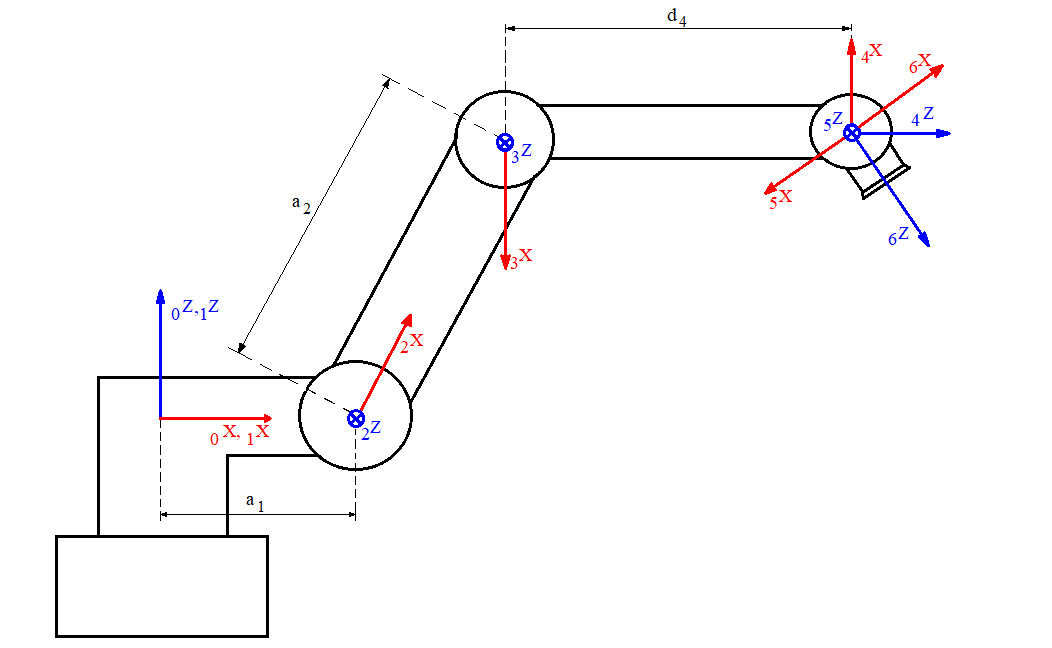
\includegraphics[width=\textwidth]{kinematyka_wymiary.png}
	\caption{Schematyczny rysunek manipulatora z zaznaczonymi osiami $_i z$ i $_i x$ oraz parametrami $a_i$ i $d_i$}
	\label{fig::kinematyka}
\end{figure}

\begin{figure}[H]
	\centering
	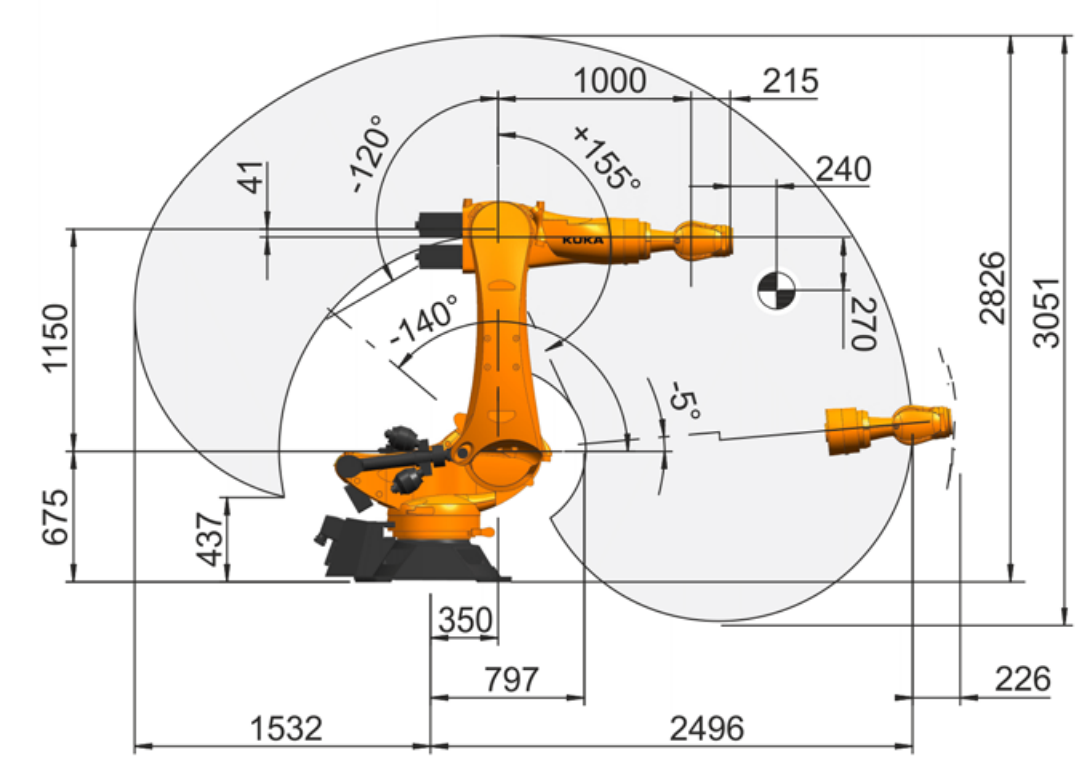
\includegraphics[width=\textwidth]{KR120_R2500.png}
	\caption{Rzut izometryczny robota KUKA KR120 R2500}
	\label{fig::robot_kr120}
\end{figure}



W tabeli \ref{tab::parametry_DH} przedstawiono parametry Denavita-Hartenberga dla danego robota.

\begin{table}[H]
\centering
\caption{Parametry Denavita-Hartenberga}
\label{tab::parametry_DH}
\begin{tabular}{|l|c|c|c|c|}
\hline
$i$	&$a_{i-1}$	&$\alpha_{i-1}$	&$d_i$	&$\theta_i$	\\ \hline
1	&0		&0			&0		&$\theta_1$  \\ \hline
2	&$a_1$	&$-\pi/2$		&0		&$\theta_2$  \\ \hline
3	&$a_2$	&0			&0		&$\theta_3$  \\ \hline
4	&0		&$\pi/2$		&$d_4$	&$\theta_4$  \\ \hline
5	&0		&$\pi/2$		&0		&$\theta_5$  \\ \hline
6	&0		&$\pi/2$		&0		&$\theta_6$  \\ \hline
\end{tabular}
\end{table}

%%%%%%%%%%%%%%%%%%%%%%%%%%%%%%%%%%%%%%%%%%%%%%%%%%%%%%%%%%%%%%%%%%%%%%%%%%%%
\subsection{Rozwiązanie prostego zadania kinematyki (PZK)}

Dla skrócenia zapisów przyjęto następujące oznaczenia:
\[ c_i = cos\theta_i, s_i = sin\theta_i, c_{i j} = cos(\theta_i+\theta_j), s_{i j} = sin (\theta_i + \theta_j) \]

Macierze opisujące człony/złącza:
\[
_{i}^{i-1}T=
\begin{bmatrix}
c_i	&-s_i	&0	&a_{i-1}	\\
s_i c\alpha_{i-1}	&c_i c\alpha_{i-1}	&-s\alpha_{i-1}	&-d_i s\alpha_{i-1}	\\
s_i s\alpha_{i-1}	&c_i s\alpha_{i-1}	& c\alpha_{i-1}	&d_i c\alpha_{i-1}	\\
0	&0	&0	&1	
 \end{bmatrix}
\]

\[
_{1}^{0}T=
\begin{bmatrix}
c_1	&-s_1	&0	&0	\\
s_1	&c_1	&0	&0	\\
0	&0	&1	&0	\\
0	&0	&0	&1	
 \end{bmatrix}
\]

\[
_{2}^{1}T=
\begin{bmatrix}
c_2	&-s_2	&0	&a_1	\\
0	&0	&1	&0	\\
-s_2	&-c_2	&0	&0	\\
0	&0	&0	&1	
 \end{bmatrix}
\]

\[
_{3}^{2}T=
\begin{bmatrix}
c_3	&-s_3	&0	&a_2	\\
s_3	&c_3	&0	&0	\\
0	&0	&1	&0	\\
0	&0	&0	&1	
 \end{bmatrix}
\]

\[
_{4}^{3}T=
\begin{bmatrix}
c_4	&-s_4	&0	&0	\\
0	&0	&-1	&-d_4	\\
s_4	&c_4	&0	&0	\\
0	&0	&0	&1
 \end{bmatrix}
\]

\[
_{5}^{4}T=
\begin{bmatrix}
c_5	&-s_5	&0	&0	\\
0	&0	&-1	&0	\\
s_5	&c_5	&0	&0	\\
0	&0	&0	&1	
 \end{bmatrix}
\]

\[
_{6}^{5}T=
\begin{bmatrix}
c_6	&-s_6	&0	&0	\\
0	&0	&-1	&0	\\
s_6	&c_6	&0	&0	\\
0	&0	&0	&1		
 \end{bmatrix}
\]

Złożenie macierzy:

\[
_{2}^{0}T= _{1}^{0}T \cdot _{2}^{1}T = 
\begin{bmatrix}
c_2c_2	&- c_1s_2	&-s_1	&a_1c_1	\\
s_1c_2	&-s_1s_2	&c_1	&a_1s_1	\\
-s_2	&-c_2	&0	&0	\\
0	&0	&0	&1	
 \end{bmatrix}
\]

\[
_{3}^{0}T= _{2}^{0}T \cdot _{3}^{2}T = 
\begin{bmatrix}
c_1c_{23}	&-c_1s_{23}	&-s_1	&c_1(a_2c_2+a_1)	\\
s_1c_{23}	&-s_1s_{23}	&c_1	&s_1(a_2c_2+a_1)	\\
-s_{23}	&-c_{23}	&0	&-a_2s_2	\\
0		&0		&0	&1	
 \end{bmatrix}
\]

\[
_{4}^{0}T= _{3}^{0}T \cdot _{4}^{3}T = 
\begin{bmatrix}
c_1c_{23}c_4 - s_1s_4	&-c_1c_{23}s_4 - s_1c_4	&c_1s_{23}	&c_1(d_4s_{23}+a_2c_2+a_1)	\\
s_1c_{23}c_4+c_1s_4	&-s_1c_{23}s_4+c_1c_4	&s_1s_{23}	&s_1(d_4s_{23}+a_2c_2+a_1)	\\
-s_{23}c_4	&s_{23}s_4	&c_{23}	&d_4c_{23}-a_2s_2	\\
0	&0	&0	&1
 \end{bmatrix}
\]

\[
_{5}^{0}T= _{4}^{0}T \cdot _{5}^{4}T = 
\begin{bmatrix}
c_5(c_1c_{23}c_4-s_1s_4)+c_1s_{23}s_5	&-s_5(c_1c_{23}c_4-s_1s_4)+c_1s_{23}c_5	&c_1c_{23}s_4+s_1c_4	&c_1(d_4s_{23}+a_2c_2+a_1)	\\
c_5(s_1c_{23}c_4+c_1s_4)+s_1s_{23}s_5	&-s_5(s_1c_{23}c_4+c_1s_4)+s_1s_{23}c_5	&s_1c_{23}s_4-c_1c_4	&s_1(d_4s_{23}+a_2c_2+a_1)	\\
-s_{23}c_4c_5+c_{23}s_5	&s_{23}c_4s_5+c_{23}c_5	&-s_{23}s_4	&d_4c_{23}-a_2s_2	\\
0	&0	&0	&1	
 \end{bmatrix}
\]
\pagebreak

\[_{6}^{0}T= _{5}^{0}T \cdot _{6}^{5}T = \]
\[ =
\left [
  \begin{tabular}{cc}
$c_6(c_5(c_1c_{23}c_4-s_1s_4)+c_1s_{23}s_5)+s_6(c_1c_{23}s_4+s_1c_4)	$	&$-s_6(c_5(c_1c_{23}c_4-s_1s_4)+c_1s_{23}s_5)+c_6(c_1c_{23}s_4+s_1c_4)$ 	\\
$c_6(c_5(s_1c_{23}c_4+c_1s_4)+s_1s_{23}s_5)+s_6(s_1c_{23}s_4-c_1c_4)	$	&$-s_6(c_5(s_1c_{23}c_4+c_1s_4)+s_1s_{23}s_5)+c_6(s_1c_{23}s_4-c_1c_4)$	\\
$c_{23}s_5c_6-s_{23}(c_4c_5c_6+s_4s_6)						$	&$s_{23}(c_4c_5s_6-s_4c_6)-c_{23}s_5s_6$		   					\\
$0												$	&$0$												
  \end{tabular}
\right .
\]
\[
\left .
  \begin{tabular}{cc}
$s_5(c_1c_{23}c_4-s_1s_4)-c_1s_{23}c_5	$	&$c_1(d_4s_{23}+a_2c_2+a_1)$ \\
$s_5(s_1c_{23}c_4+c_1s_4)-s_1s_{23}c_5	$	&$s_1(d_4s_{23}+a_2c_2+a_1)$ \\
$-s_{23}c_4s_5-c_{23}c_5			$	&$d_4c_{23}-a_2s_2$		   \\
$0							$	&$1$												
  \end{tabular}
\right ]
\]

%\[
%\begin{bmatrix}
%c_6(c_5(c_1c_{23}c_4-s_1s_4)+c_1s_{23}s_5)+s_6(c_1c_{23}s_4+s_1c_4)	&-s_6(c_5(c_1c_{23}c_4-s_1s_4)+c_1s_{23}s_5)+c_6(c_1c_{23}s_4+s_1c_4)	&s_5(c_1c_{23}c_4-s_1s_4)-c_1s_{23}c_5	&c_1(d_4s_{23}+a_2c_2+a_1)	\\
%c_6(c_5(s_1c_{23}c_4+c_1s_4)+s_1s_{23}s_5)+s_6(s_1c_{23}s_4-c_1c_4)	&-s_6(c_5(s_1c_{23}c_4+c_1s_4)+s_1s_{23}s_5)+c_6(s_1c_{23}s_4-c_1c_4)	&s_5(s_1c_{23}c_4+c_1s_4)-s_1s_{23}c_5	&s_1(d_4s_{23}+a_2c_2+a_1)	\\
%c_{23}s_5c_6-s_{23}(c_4c_5c_6+s_4s_6)						&s_{23}(c_4c_5s_6-s_4c_6)-c_{23}s_5s_6						&-s_{23}c_4s_5-c_{23}c_5			&d_4c_{23}-a_2s_2	\\
%0												&0												&0							&1		
%\end{bmatrix}
%\]

%%%%%%%%%%%%%%%%%%%%%%%%%%%%%%%%%%%%%%%%%%%%%%%%%%%%%%%%%%%%%%%%%%%%%%%%%%%%
\subsection{Rozwiązanie odwrotnego zadania kinematyki (OZK)}

Zdefiniowano następujące macierze po\'srednie:
\[
_{3}^{1}T= _{2}^{1}T \cdot _{3}^{2}T = 
\begin{bmatrix}
c_{23}	&-s_{23}	&0	&a_2c_2+a_1	\\
0		&0		&1	&0			\\
-s_{23}	&-c_{23}	&0	&-a_2s_2		\\
0		&0		&0	&1	
 \end{bmatrix}
\]

\[
_{4}^{1}T= _{3}^{1}T \cdot _{4}^{3}T = 
\begin{bmatrix}
c_{23}c_4	&-c_{23}s_4	&s_{23}	&d_4s_{23}+a_2c_2+a_1	\\
s_4		&c_4		&0		&0			\\
-s_{23}c_4	&s_{23}s_4	&c_{23}	&d_4c_{23}-a_2s_2		\\
0		&0		&0		&1	
 \end{bmatrix}
\]

\[
_{6}^{4}T= _{5}^{4}T \cdot _{6}^{5}T = 
\begin{bmatrix}
c_5c_6	&-c_5s_6	&s_5	&0	\\
-s_6		&-c_6		&0	&0	\\
s_5c_6	&-s_5s_6	&-c_5	&0	\\
0		&0		&0	&1	
 \end{bmatrix}
\]

Stąd:
\[
_{6}^{1}T= _{4}^{1}T \cdot _{6}^{4}T = 
\begin{bmatrix}
c_{23}(c_4c_5c_6+s_4s_6)+s_{23}s_5c_6	&c_{23}(s_4c_6-c_4c_5s_6)-s_{23}s_5s_6	&c_{23}c_4s_5-s_{23}c_5	&d_4s_{23}+a_2c_2+a_1	\\
s_4c_5c_6-c_4s_6					&-s_4c_5s_6-c_4c_6				&s_4s_5				&0				\\
-s_{23}(c_4c_5c_6+s_4s_6)+c_{23}s_5c_6	&s_{23}(c_4c_5s_6-s_4c_6)-c_{23}s_5s_6	&-s_{23}c_4s_5-c_{23}c_5	&d_4c_{23}-a_2s_2	\\
0							&0							&0					&1	
 \end{bmatrix}
\]

Następnie do rozwiązania odwrotnego zadania kinematyki posłużono się zależno\'sciami:
\[_n^0T = _n^0T_d,\]
w którym lewa strona oznacza wynik PZK za\'s prawa stałe. Następnie:
\[_1^0T^{-1}~ _n^0T = _1^0T^{-1}~ _n^0T_d\]
\[_n^0T~ _n^{n-1}T^{-1} = _n^0T_d ~ _n^{n-1}T^{-1}\]
poszukuje się elementów dających $f(\theta_i)=$ const, które po znalezieniu są traktowane jako wielko\'sci znane.
Macierz stałych $_n^0T_d$ jest następująca:
\[
_n^0T_d =
\begin{bmatrix}
r_{11}	&r_{12}	&r_{13}	&p_x	\\
r_{21}	&r_{22}	&r_{23}	&p_y	\\
r_{31}	&r_{32}	&r_{33}	&p_z	\\
0		&0		&0		&1	
 \end{bmatrix}, 
\]
W celu porównania wyznaczonej wcze\'sniej macierzy $_{6}^{1}T$ należy wyznaczyć poniższy iloczyn macierzowy:
\[
_1^0T^{-1}~ _n^0T_d =
\begin{bmatrix}
c_1r_{11}+s_1r_{21}	&c_1r_{12}+s_1r_{22}	&c_1r_{13}+s_1r_{23}	&c_1p_x+s_1p_y	\\
c_1r_{21}-s_1r_{11}	&c_1r_{22}-s_1r_{12}	&c_1r_{23}-s_1r_{13}	&c_1p_y-s_1p_x	\\
r_{31}			&r_{32}			&r_{33}			&p_z	\\
0				&0				&0				&1	
 \end{bmatrix}
\]
Zgodnie ze wzorem:
\[_1^0T^{-1}~ _n^0T_d = _{6}^{1}T\]
Porównując kolejne elementy macierzy można wyznaczyć kąty $\theta_i$.

Wybieramy element $_6^1T_{24} \Rightarrow c_1p_y - s_1p_x = 0 \Rightarrow c_1p_y=s_1p_x \Rightarrow \dfrac{s_1}{c_1}=\dfrac{p_y}{p_x} \Rightarrow \theta_1 = arctan \left ( \dfrac{p_y}{p_x} \right )$

W celu znalezienia kąta $\theta_2$ wybrano elementy $_6^1T_{14}$ i $_6^1T_{34}$ (ze względu, iż występują w nich tylko dwa nieznane kąty $\theta_2$ i $\theta_2$:
\[
\begin{cases}
c_1p_x+s_1p_y = d_4s_{23}+a_2c_2+a_1\\
p_z = d_4c_{23}-a_2s_2
\end{cases}
\]
Po przekształceniu
\[
\begin{cases}
c_1p_x+s_1p_y-a_1 = d_4s_{23}+a_2c_2\\
p_z = d_4c_{23}  - a_2s_2 ,
\end{cases}
\]
otrzymujemy równania, które po lewej stronie zawierają wyrażenia stałe. Zatem w celu uproszczenia zapisu wprowadzono następujące podstawienia:

\begin{align*}
E &= c_1p_x+s_1p_y-a_1\\
F &= p_z
\end{align*}
Otrzymujemy standardowy układ równań:
\[
\begin{cases}
E - a_2c_2 = d_4s_{23}\\
F +a_2s_2 = d_4c_{23}
\end{cases}
\]

Podnosząc równania obustronie do kwadratu i dodając stronami otrzymujemy:
\[
E^2 + F^2 + a_2^2(c_2^2+s_2^2)  -2Ea_2c_2 + 2Fa_2s_2=d_4^2(s_{23}^2+c_{23}^2)
\]
\[
E^2 + F^2 + a_2^2  -2Ea_2c_2 + 2Fa_2s_2=d_4^2
\]
\[
E^2 + F^2 + a_2^2 - d_4^2 =  2Ea_2c_2 - 2Fa_2s_2
\]
Po lewej stronie równania mamy wyrażenie stałe, więc stosując podstawienie:
\[
K=E^2 + F^2 + a_2^2 - d_4^2,
\]
otrzymujemy:
\[
K=2Ea_2c_2 - 2Fa_2s_2 .
\]
Wprowadzając współrzędne biegunowe:
\[
\begin{cases}
G=2Ea_2=rs(\varphi)\\
H=- 2Fa_2=rc(\varphi)
\end{cases}
\]
\[
\begin{cases}
r=\sqrt{G^2+F^2} \\
\varphi = arctan \Big(\frac{G}{H}\Big) ,
\end{cases}
\]
równanie przyjmuje następującą postać:
\[
K=rs(\varphi)c_2 + rc(\varphi)s_2 = r(s(\varphi)c_2 + c(\varphi)s_2) = rs(\varphi+\theta_2) \Rightarrow \dfrac{K}{r}=s(\varphi+\theta_2) 
\]
Zatem mamy układ równań:
\[
\begin{cases}
s(\varphi+\theta_2) =\dfrac{K}{r}=\\
c(\varphi+\theta_2)= \pm \sqrt{1-\Big(\dfrac{K}{r}\Big)^2} ,
\end{cases}
\]
który po podzieleniu stronami i zastosowaniu funkcji $arctan$ pozwala na wyznaczenie warto\'sci kąta $\theta_2$:
\[
\theta_2 = arctan \Bigg( \dfrac{\frac{K}{r}}{\pm \sqrt{1-\Big(\frac{K}{r}\Big)^2}}\Bigg) - arctan \Big(\frac{G}{H}\Big)
\]

Korzystając ponownie z układu równań:
\[
\begin{cases}
E - a_2c_2 = d_4s_{23}\\
F +a_2s_2 = d_4c_{23},
\end{cases}
\]
wyznaczamy kąt $\theta_3$ poprzez podział stronami i zastosowanie funkcji $arctan$:
\[
\theta_2+\theta_3 = arctan \Bigg(\dfrac{E - a_2c_2}{F +a_2s_2} \Bigg)
\]
\[
\theta_3 = arctan \Bigg(\dfrac{E - a_2c_2}{F +a_2s_2} \Bigg) - \theta_2
\]

Mając wyznaczone kąty $\theta_1,\theta_2,\theta_3$ można wyznaczyć kąt $\theta_5$ przy wykorzystaniu elementów $_6^1T_{13}$ i $_6^1T_{33}$:
\[
\begin{cases}
c_{23}c_4s_5-s_{23}c_5=c_1r_{13}+s_1r_{23}\\
-s_{23}c_4s_5-c_{23}c_5=r_{33}
\end{cases}
\]
Po prawej stronie równań występują wyrażenia stałe zatem stosując podstawienie:
\begin{align*}
L&=c_1r_{13}+s_1r_{23}\\
M&=-r_{33},
\end{align*}
otrzymujemy:
\[
\begin{cases}
c_{23}c_4s_5-s_{23}c_5=L\\
s_{23}c_4s_5+c_{23}c_5=M
\end{cases}
\]
Z drugiego równania wyznaczamy:
\[
c_4s_5=\dfrac{M-c_{23}c_5}{s_{23}}
\]
Podstawiając do pierwszego równania uzyskujemy:
\[
c_{23}\dfrac{M-c_{23}c_5}{s_{23}}-s_{23}c_5=L
\]
Mnożąc obustronnie przez $s_{23}$ uzyskujemy:
\[
c_{23}M-c_{23}^2c_5-s_{23}^2c_5=s_{23}L
\]
\[
c_{23}M-c_5=s_{23}L
\]
\[
c_{23}M-s_{23}L=c_5
\]
Taki sam wzór uzyskuję się wyznaczając $c_4s_5$ z pierwszego równania stosując dzielenie przez $c_{23}$.
Zatem kąt $\theta_5$  ma warto\'sć:
\[
\theta_5=arccos(c_{23}M-s_{23}L)
\]

Następnie można wyznaczyć kąt $\theta_4$ przy wykorzystaniu elementu $_6^1T_{23}$:
\[
s_4s_5=c_1r_{23}-s_1r_{13}
\]
\[
\theta_4=arcsin\Big(\dfrac{c_1r_{23}-s_1r_{13}}{s_5}\Big), s_5 \neq 0
\]

Osobliwo\'sć, gdy $s_5=0(\theta_5=0$ lub $ \theta_5=\pi) \Rightarrow$
\[
_{6}^{1}T= 
\begin{bmatrix}
\pm c_{23}c(\theta_4 \mp \theta_6)		&c_{23}s(\theta_4 \mp \theta_6)	&\mp s_{23}			&d_4s_{23}+a_2c_2+a_1	\\
\pm s(\theta_4 \mp \theta_6)			&-c(\theta_4 \mp \theta_6)		&0				&0				\\
-s_{23}(\pm c(\theta_4 \mp \theta_6))		&-s_{23}s(\theta_4 \mp \theta_6)	&\mp c_{23}			&d_4c_{23}-a_2s_2	\\
0							&0						&0				&1	
 \end{bmatrix}
\]
Biorąc pod uwagę elementy $_6^1T_{11}$ i $_6^1T_{12}$ i dzieląc je przez siebie otrzymujemy:
\[
\dfrac{_6^1T_{12}}{_6^1T_{11}}=\dfrac{\pm s(\theta_4 \mp \theta_6)}{\pm c_{23}c(\theta_4 \mp \theta_6)}=\dfrac{c_1r_{21}-s_1r_{11}}{c_1r_{11}+s_1r_{21}}
\]
\[
\dfrac{\pm s(\theta_4 \mp \theta_6)}{\pm c(\theta_4 \mp \theta_6)}=\dfrac{c_{23}(c_1r_{21}-s_1r_{11})}{c_1r_{11}+s_1r_{21}}
\]
\[
(\theta_4 \mp \theta_6)=arctan \Bigg(\dfrac{c_{23}(c_1r_{21}-s_1r_{11})}{c_1r_{11}+s_1r_{21}}\Bigg)
\]
Zatem można przyjąć (przy $s_5=0$), iż warto\'sć kąta $\theta_4$ w danej chwili może równać się warto\'sci tego kąta z chwili poprzedniej.

Do wyznaczenia kąta $\theta_6$ zostaną wykorzystane elementy $_6^1T_{21}$ i $_6^1T_{22}$
\[
\begin{cases}
s_4c_5c_6-c_4s_6=c_1r_{21}-s_1r_{11}\\
-s_4c_5s_6-c_4c_6=c_1r_{22}-s_1r_{12}
\end{cases}
\]
Po prawej stronie mamy wyrażenia stałe, zatem stosując podstawienie
\[
\begin{cases}
N=c_1r_{21}-s_1r_{11}\\
P=c_1r_{22}-s_1r_{12},
\end{cases}
\]
otrzymujemy:
\[
\begin{cases}
s_4c_5c_6-c_4s_6=N\\
-s_4c_5s_6-c_4c_6=P
\end{cases}
\]
\[
\begin{cases}
s_4c_5c_6=N+c_4s_6\\
-s_4c_5s_6=P+c_4c_6
\end{cases}
\]
Po podniesieniu do kwadratu i dodaniu stronami otrzymujemy:
\[
s_4^2c_5^2=N^2+P^2+2Nc_4s_6+2Pc_4c_6+c_4^2
\]
\[
s_4^2c_5^2-N^2-P^2-c_4^2=2Nc_4s_6+2Pc_4c_6
\]
Po lewej stronie równania mamy wyrażenie stałe, więc stosując podstawienie:
\[
D=s_4^2c_5^2-N^2-P^2-c_4^2,
\]
otrzymujemy:
\[
D=2Nc_4s_6+2Pc_4c_6 .
\]
Wprowadzając współrzędne biegunowe:
\[
\begin{cases}
U=2Pc_4=Rs(\varphi)\\
W=2Nc_4=Rc(\varphi)
\end{cases}
\]
\[
\begin{cases}
R=\sqrt{U^2+W^2} \\
\varphi = arctan \Big(\frac{U}{W}\Big) ,
\end{cases}
\]
równanie przyjmuje następującą postać:
\[
D=Rs(\varphi)c_6 + Rc(\varphi)s_6 = R(s(\varphi)c_6 + c(\varphi)s_6) = Rs(\varphi+\theta_6) \Rightarrow \dfrac{D}{R}=s(\varphi+\theta_6) 
\]

Zatem mamy układ równań:
\[
\begin{cases}
s(\varphi+\theta_6) =\dfrac{D}{R}\\
c(\varphi+\theta_6)= \pm \sqrt{1-\Big(\dfrac{D}{R}\Big)^2} ,
\end{cases}
\]
który po podzieleniu stronami i zastosowaniu funkcji $arctan$ pozwala na wyznaczenie warto\'sci kąta $\theta_2$:
\[
\theta_6 = arctan \Bigg( \dfrac{\frac{D}{R}}{\pm \sqrt{1-\Big(\frac{D}{R}\Big)^2}}\Bigg) - arctan \Big(\frac{U}{W}\Big)
\]
Wybór wła\'sciwego rozwiązania spo\'sród wielu otrzymywanych dokonywany jest na podstawie założenia o ciągło\'sci trajektorii. Wła\'sciwe rozwiązanie jest najbliższe akutalnej pozycji ramienia.


\end{document}